%%%% Paramétrage du TD %%%%
\def\xxactivite{Révisions \ifprof -- Corrigé \else \fi} % \normalsize \vspace{-.4cm}
\def\xxauteur{\textsl{Xavier Pessoles}}


\def\xxnumchapitre{Révision cinématique \vspace{.2cm}}
\def\xxchapitre{\hspace{.12cm} Résolution cinématique}
\def\xxonglet{\textsf{Rév -- Stat}}
\def\xxactivite{TD 02}
\def\xxauteur{\textsl{Xavier Pessoles}}

\def\xxpied{%
Révision cinématique \\
Fiche  2 -- \xxactivite%
}


\def\xxtitreexo{Magic Arms}
\def\xxsourceexo{\hspace{.2cm} \footnotesize{Florestan Mathurin}}


\def\xxcompetences{%
\textsl{%
\textbf{Savoirs et compétences :}\\} \vspace{-.5cm}
%\begin{itemize}
%\item \textit{Res2.C18} : principe fondamental de la statique;
%\item \textit{Res2.C19} : équilibre d’un solide, d’un ensemble de solides;
%\item \textit{Res2.C20} : théorème des actions réciproques.
%\end{itemize}
}


\def\xxfigures{
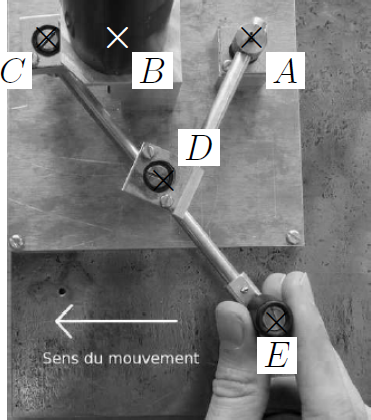
\includegraphics[width=.7\textwidth]{fig_00}
}%figues de la page de garde

\input{\repStyle/pagegarde_TD}

\setlength{\columnseprule}{.1pt}

\pagestyle{fancy}
\thispagestyle{plain}

\vspace{5cm}


\def\columnseprulecolor{\color{ocre}}
\setlength{\columnseprule}{0.4pt} 

%%%%%%%%%%%%%%%%%%%%%%%

\setcounter{numques}{0}

\ifprof
\else
\begin{multicols}{2}
\fi


La manège Magic Arms dont la modélisation ainsi qu'un extrait de cahier des charges fonctionnel est composé d'une structure métallique d'environ \SI{12}{m} de haut avec deux bras mobiles. Les passagers s'assoient sur 39 pièces disposées sur une plate-forme tournante. Dès que tous les passagers sont assis et attachés, la nacelle tourne autour de son axe, le bras principal (bras \textbf{1}) et le bras secondaires (bras \textbf{2}), liés l'un à l'autre au début du cycle, commencent à tourner. Après 9 secondes, le maximum de hauteur est atteint et les deux bras se désindexent et se mettent à tourner indépendamment l'un de l'autre. Tous les mouvements sont pilotés par ordinateur. 

\begin{center}
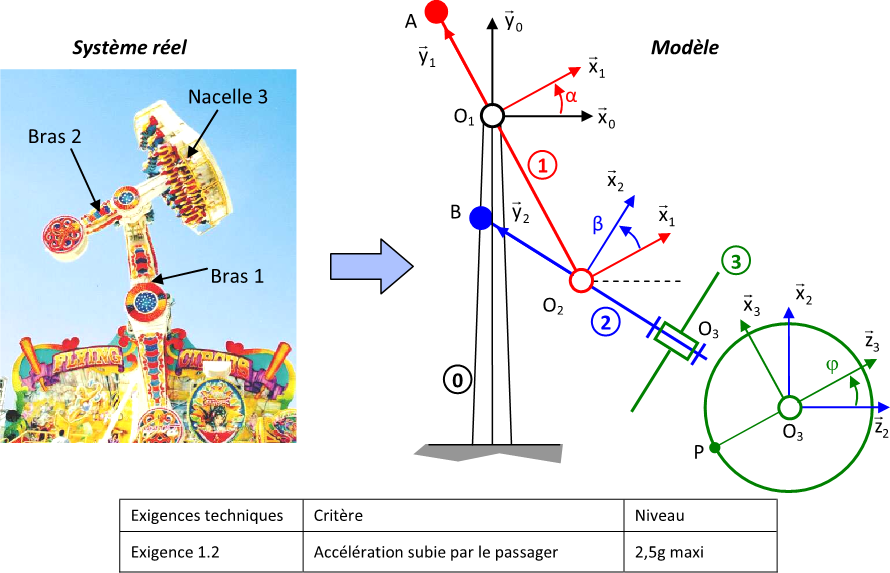
\includegraphics[width=\linewidth]{img1}
\end{center}

Le manège, schématisé ci-dessus, comporte :
\begin{itemize}
\item un bras principal \textbf{1} assimilé à une barre $AO_1O_2$. Il est en liaison pivot parfait d'axe $(O_1,\vect{z_1})$ caractérisée par le paramètre $\alpha$ avec le bâti \textbf{0}. On pose $\vect{O_1O_2}=-l_1\vect{y_1}$;
\item un bras secondaire 2 assimilé à une barre $BO_2O_3$. Il est en liaison pivot parfait d'axe $(O_2,\vect{z_2})$ caractérisée par le paramètre $\beta$ avec le bras principal \textbf{1}. On pose $\vect{O_2O_3}=-l_2\vect{y_2}$;
\item une nacelle \textbf{2} assimilée à un disque de centre $O_3$ et de rayon $R$. Elle est en liaison parfaite d'axe $(O_3,\vect{y_2})$ caractérisée par le paramètre $\varphi$ avec le bras \textbf{2}. On s'intéresse plus particulièrement à un passager considéré comme un point matériel $P$ tel que $\vect{O_3P}=-R\vect{z_3}$.
\end{itemize}

\question{Construire les figures planes associées au schéma cinématique.}
\ifprof

\begin{corrige}
%\couleursfigureplane{black}{red}
%\figureplanerep{x_0}{x_1}{y_0}{y_1}{z_0}{\alpha}{0}{1}{3}
%\couleursfigureplane{red}{blue}
%\figureplanerep{x_1}{x_2}{y_1}{y_2}{z_0}{\beta}{1}{2}{3}
%\couleursfigureplane{blue}{green}
%\figureplanerep{z_0}{z_3}{x_2}{x_3}{y_2}{\varphi}{2}{3}{3}

\end{corrige}\else\fi

\question{Calculer $\vecto{1}{0}$, $\vecto{2}{1}$ et $\vecto{3}{2}$.}
\ifprof
\begin{corrige}
\begin{align*}
\vecto{1}{0}&=\dot\alpha\vect{z_0}\\
\vecto{2}{1}&=\dot\beta\vect{z_0}\\
\vecto{3}{2}&=\dot\varphi\vect{y_2}\\
\end{align*}
\end{corrige}\else\fi

%\vspace{.3cm}

%On admet que $\vecto{3}{0}=\vecto{3}{2}+\vecto{2}{1}+\vecto{1}{0}$.

\question{Calculer $\vecto{2}{0}$ et $\vecto{3}{0}$.}
\ifprof
\begin{corrige}
\begin{align*}
\vecto{2}{0}&=\vecto{2}{1}+\vecto{1}{0}\\
	&=(\dot\alpha+\dot\beta)\vect{z_0}\\
\vecto{3}{0}&=\vecto{3}{2}+\vecto{2}{0}\\
	&=(\dot\alpha+\dot\beta)\vect{z_0}+\dot\varphi\vect{y_2}
\end{align*}

\end{corrige}\else\fi

\question{Calculer les produits vectoriels suivants : $\vect{z_2}\wedge\vect{z_3}$,
$\vect{x_3}\wedge\vect{x_2}$, $\vect{x_3}\wedge\vect{z_2}$,
$\vect{z_2}\wedge\vect{z_1}$, $\vect{x_2}\wedge\vect{x_0}$,
$\vect{x_3}\wedge\vect{z_0}$.}
\ifprof
\begin{corrige}

\begin{align*}
\vect{z_2} \wedge \vect{z_3} &=\sin\varphi \vect{y_2}\\
\vect{x_3} \wedge\vect{x_2} &= -\sin\varphi \vect{y_2}\\
\vect{x_3} \wedge \vect{z_2}&= -\sin\left(\dfrac{\pi}{2}+\varphi\right)\vect{y_2}\\
	&=-\cos\varphi\vect{y_2}\\
\vect{z_2} \wedge \vz1 &= \vec{0}\\
\vect{x_2} \wedge \vx0 &= \left(\cos\beta\vx1+\sin\beta\vy1\right)\wedge\vx0\\
	&=-\cos\beta\sin\alpha\vect{z_0} - \sin\beta\sin\left(\dfrac{\pi}{2}+\alpha\right)\vect{z_0}\\
	&=(-\cos\beta\sin\alpha-\sin\beta\cos\alpha)\vect{z_0}\\
	&=-\sin(\beta+\alpha)\vect{z_0}\\
\vect{x_3}\wedge\vect{z_0} &= -\sin\left(\dfrac{\pi}{2}+\varphi\right)\vect{y_2}\\
	&=-\cos\varphi\vect{y_2}
\end{align*}

\end{corrige}\else\fi

\question{Calculer $\vectv{O_2}{2}{0}$, $\vectv{O_3}{3}{0}$ et $\vectv{P}{3}{0}$.}
\ifprof
\begin{corrige}
\begin{align*}
\vectv{O_2}{2}{0}&=\vectv{O_2}{2}{1}+\vectv{O_2}{1}{0}\\
	&=\vectv{O_1}{1}{0}+\vecto{1}{0}\wedge\gv{O_1 O_2}\\
	&= \dot\alpha\vect{z_0} \wedge (-l_1 \vy1) \\
{\vectv{O_2}{2}{0}}{= l_1\dot\alpha\vx1}\\
\vectv{O_3}{3}{0}&=\vectv{O_3}{3}{2}+\vectv{O_3}{2}{0}\\
	&=\vectv{O_2}{2}{0}+\vecto{2}{0}\wedge \gv{O_2 O_3}\\
	&=l_1\dot\alpha\vx1+(\dot\alpha+\dot\beta)\vect{z_0}\wedge (-l_2 \vect{y_2})\\
{\vectv{O_3}{3}{0}{=l_1\dot\alpha\vx1+l_2(\dot\alpha+\dot\beta)\vect{x_2}}\\
\vectv{{P}{3}{0}&=\vectv{{O_3}{3}{0}+\vecto{3}{0}\wedge\gv{O_3 P}\\	&=l_1\dot\alpha\vx1+l_2(\dot\alpha+\dot\beta)\vect{x_2}+ \left((\dot\alpha+\dot\beta)\vect{z_0}+\dot\varphi\vect{y_2}\right)\wedge(-R\vect{z_3})\\
{\vectv{P}{3}{0}{=l_1\dot\alpha\vx1+l_2(\dot\alpha+\dot\beta)\vect{x_2}-R\sin\varphi(\dot\alpha+\dot\beta)\vect{y_2}-R\dot\varphi\vect{x_3}}
\end{align*}
\end{corrige}\else\fi

\vspace{.3cm}

On donne l'évolution des vitesses angulaires des moteurs du manège en fonction du temps.
\begin{center}
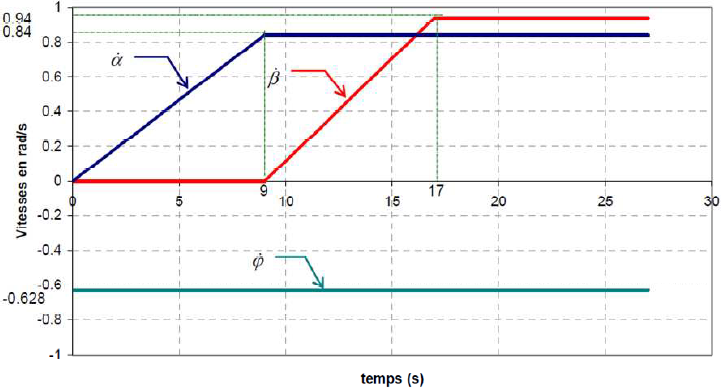
\includegraphics[width=\linewidth]{img2}
\end{center}

\question{\label{lab} Déterminer les valeurs des paramètres $\dot{\alpha}$, $\dot{\beta}$ et $\dot{\varphi}$
puis l'expression analytique des positions angulaires $\alpha(t)$ et $\beta(t)$ et $\varphi(t)$ dans l'intervalle de temps $[17;27]$ secondes en sachant qu'à l'instant $t=\SI{17}{s}$, on a $\alpha=\SI{10,5}{rad}$, $\beta=\SI{3,76}{rad}$ et $\varphi=-\SI{10,676}{rad}$.}
\ifprof
\begin{corrige}

Dans l'intervalle de temps compris entre 17 et 27 secondes, les vitesses angulaires sont constantes.

$$
\systeq{
{\dot\alpha}{=\SI{0,84}{rad/s}}\\
{\dot\beta}{=\SI{0,94}{rad/s}}\\
{\dot\varphi}{=-\SI{0,628}{rad/s}}
}
$$

Ainsi, par intégration :
\begin{align*}
\alpha (t)-\alpha(17)&=\int_{17}^t \dot\alpha d\tau \\
%\alpha (t)-10,5&=0,84(t-17) \\
%{\alpha (t) }{= 0,84(t-17) + 10,5}\\	
%\beta (t)-\beta(17)&=\int_{17}^t \dot\beta d\tau \\
%\beta (t)-3,76&=0,94(t-17) \\
%{\beta (t) }{= 0,94(t-17) + 3,76}	\\
%\varphi (t)-\varphi(17)&=\int_{17}^t \dot\varphi d\tau \\
%\varphi (t)+10,676&=-0,628(t-17) \\
%{\varphi (t) }{= -0,628(t-17) -10,676}	\\
\end{align*}
\end{corrige}\else\fi

\question{Déterminer les valeurs numériques à l'instant $t_1=19,8\; s$ de $\alpha$, $\beta$ et $\varphi$.}
\ifprof
\begin{corrige}

Pour $t=19,8$ s,
\[
\systeq{
\alpha&=0,84 \times (19,8-17) + 10,5=\boxed{12,85\text{ rad}}\\
\beta&=0,94\times (19,8-17) +3,76 = \boxed{6,39\text{ rad}}\\
\varphi &= -0,628\times (19,8-17) -10,676 =\boxed{12,43\text{ rad}}
}
\]

\end{corrige}\else\fi

\question{On pose $\vectv{P}{3}{0}=V_{x2}\vect{x_2}+V_{y2}\vect{y_2}+V_{z2}\vect{z_2}$. Déterminer les expressions littérales de $V_{x2}$, $V_{x2}$, $V_{z2}$ puis les valeurs numériques de à $t_1=19,8\;s.$} (On donne : $l_1=3,9\;m$, $l_2=2,87\;m$, $R=2,61\;m$.)
\ifprof
\begin{corrige}

Il s'agit de projeter le vecteur \vectv{{P}{3}{0} dans la base $(\vect{x_2}, \vect{y_2} ,\vect{z_0})$. En effet, le vecteur $\vect{z_2}$ est identique au vecteur $\vect{z_0}$.
\begin{align*}
\vectv{{P}{3}{0}&=V_{x2}\vect{x_2} +V_{y2}\vect{y_2} + V_{z2}\vect{z_0}\\
V_{x2}&=\vectv{{P}{3}{0}\cdot\vect{x_2}\\
	&=\left(l_1\dot\alpha\vx1+l_2(\dot\alpha+\dot\beta)\vect{x_2}-R\sin\varphi(\dot\alpha+\dot\beta)\vect{y_2}-R\dot\varphi\vect{x_3}\right)\cdot\vect{x_2}\\
{V_{x2}}{=l_1 \dot\alpha\cos\beta+l_2 (\dot\alpha+\dot\beta) -R \dot\varphi\cos\varphi}\\
V_{y2}&=\vectv{{P}{3}{0}\cdot\vect{y_2}\\
	&=\left(l_1\dot\alpha\vx1+l_2(\dot\alpha+\dot\beta)\vect{x_2}-R\sin\varphi(\dot\alpha+\dot\beta)\vect{y_2}-R\dot\varphi\vect{x_3}\right)\cdot\vect{y_2}\\
{V_{y2}}{=-l_1\dot\alpha\sin\beta-R\sin\varphi(\dot\alpha+\dot\beta)}\\
V_{z2}&=\vectv{{P}{3}{0}\cdot\vect{y_2}\\
	&=\left(l_1\dot\alpha\vx1+l_2(\dot\alpha+\dot\beta)\vect{x_2}-R\sin\varphi(\dot\alpha+\dot\beta)\vect{y_2}-R\dot\varphi\vect{x_3}\right)\cdot\vect{z_0}\\
{V_{z2}}{=R\dot\varphi\sin\varphi}
\end{align*}

Valeurs numériques à $t=19,8$ s :

\begin{align*}
V_{x2}&=3,9\times 0,84 \times \cos (6,39) + 2,87  \times (0,84 + 0,94) + 2,61 \times 0,628 \times \cos (12,43) \\
	&=\boxed{9,99\text{ m/s}}\\
V_{y2}&=-3,9 \times 0,84 \times \sin(6,39) - 2,61 \times \sin(12,43) \times (0,84 + 0,94)\\
	&=\boxed{-0,28\text{ m/s}}\\
V_{z2}&=-2,61\times 0,628 \times \sin(12,43) \\
	&=\boxed{-0,22 \text{ m/s}}
\end{align*}

\end{corrige}\else\fi

\question{Calculer $\vect{\Gamma\left(P\in3/0 \right)}$.}
\ifprof
\begin{corrige}

\begin{align*}
\vectg{P}{3}{0}&=\gderivect{\vectv{{P}{3}{0}}{0}\\
	&=\dfrac{\dd}{\dd t}\left( l_1\dot\alpha\vx1+l_2(\dot\alpha+\dot\beta)\vect{x_2}-R\sin\varphi(\dot\alpha+\dot\beta)\vect{y_2}-R\dot\varphi\vect{x_3} \right)_0 \\
	&=l_1 \ddot\alpha\vx1+l_1 \dot\alpha\underbrace{\derivect{\vx1}{0}}_{\dot\alpha\vy1} + l_2(\ddot\alpha + \ddot\beta)\vect{x_2}+ l_2(\dot\alpha+\dot\beta)\underbrace{\derivect{\vect{x_2}}{0}}_{(\dot\alpha+\dot\beta)\vect{y_2}}-R\dot\varphi\cos\varphi(\dot\alpha+\dot\beta)\vect{y_2}\\
	&\phantom{==}-R\sin\varphi(\ddot\alpha+\ddot\beta)\vect{y_2}-R\sin\varphi(\dot\alpha+\dot\beta)\underbrace{\derivect{\vect{y_2}}{0}}_{-(\dot\alpha+\dot\beta)\vect{x_2}}-R\ddot\varphi\vect{x_3} -R\dot\varphi\derivect{\vect{x_3}}{0}\\
\derivect{\vect{x_3}}{0}&={\derivect{\vect{x_3}}{3}}+\vecto{3}{0}\wedge\vect{x_3}\\
		&=\left((\dot\alpha+\dot\beta)\vect{z_0}+\dot\varphi\vect{y_2}\right)\wedge\vect{x_3}\\
		&=(\dot\alpha+\dot\beta)\cos\varphi\vect{y_2}-\dot\varphi\vect{z_3}
		\end{align*}
		
D'où :
\begin{align*}
\vectg{P}{3}{0}&=l_1 \ddot\alpha\vx1+l_1 \dot\alpha^2\vy1 + l_2(\ddot\alpha + \ddot\beta)\vect{x_2}+ l_2(\dot\alpha+\dot\beta)^2\vect{y_2}-2R\dot\varphi\cos\varphi(\dot\alpha+\dot\beta)\vect{y_2}\\
	& -R\sin\varphi(\ddot\alpha+\ddot\beta)\vect{y_2}+R\sin\varphi(\dot\alpha+\dot\beta)^2\vect{x_2}-R\ddot\varphi\vect{x_3} +R\dot\varphi^2\vect{z_3}
\end{align*}


\end{corrige}\else\fi

\question{Calculer $\vect{\Gamma\left(P\in3/0 \right)}$ dans l'intervalle de temps $[17;27]$ secondes pour lequel les vitesses angulaires sont constantes.}
\ifprof
\begin{corrige}

Dans le cas ou les vitesses angulaires sont constantes, les accélérations angulaires $\ddot\alpha$, $\ddot\beta$, et $\ddot\varphi$ sont nulles. L'expression de \vectg{P}{3}{0} se simplifie donc :
\begin{align*}
{\vectg{P}{3}{0}}{=l_1 \dot\alpha^2\vy1 + l_2(\dot\alpha+\dot\beta)^2\vect{y_2}-2R\dot\varphi\cos\varphi(\dot\alpha+\dot\beta)\vect{y_2}+ R\sin\varphi(\dot\alpha+\dot\beta)^2\vect{x_2} +R\dot\varphi^2\vect{z_3}}\\
\end{align*}

\end{corrige}\else\fi

\vspace{.3cm}

Le graphe ci-dessous, obtenu par simulation numérique, présente le module de la vitesse du passager $P$ par rapport au bâti 0 ainsi que le module de l'accélération du passager $P$ par rapport au bâti 0 en fonction du temps. 
\begin{center}
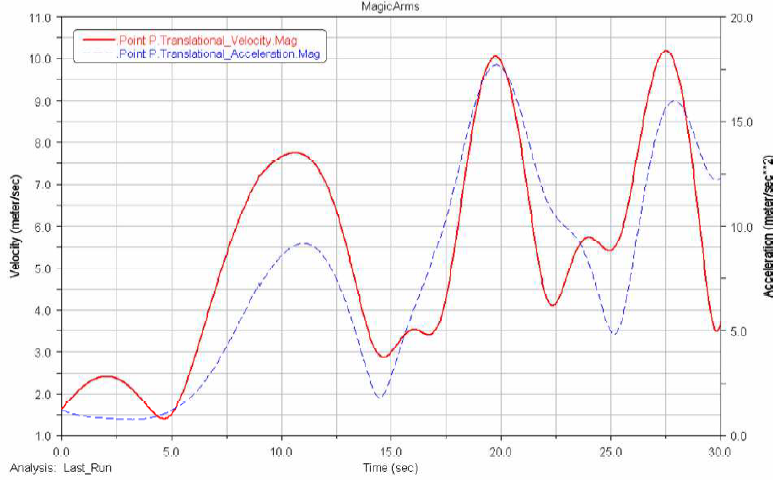
\includegraphics[width=\linewidth]{img3}
\end{center}

\question{Comparer les résultats obtenus à la question \ref{lab} à ceux du graphe pour le temps $t_1=19,8\;s.$.}
\ifprof
\begin{corrige}

Le graphe montre qu'à $t=19,8$ s, l'intensité du vecteur \vectv{{P}{3}{0} vaut 10 m/s. Or  d'après la question~8, 
\begin{align*}
\left|\left|\vectv{{P}{3}{0}\right|\right|&=\sqrt{V_{x2}^2+V_{y2}^2+V_{z2}^2}\\
	&=\sqrt{9,99^2+0,28^2+0,22^2}\\
	&=\boxed{10\text{ m/s} }
\end{align*}

On constate que le calcul littéral nous donne le même résultat que l'exploitation de la courbe.

\end{corrige}\else\fi

\question{Relever l'accélération maximale subie par le passager et conclure vis-à-vis du CdCF.}
\ifprof
\begin{corrige}
D'après la courbe de l'accélération (en pointillés), la valeur maximale de l'accélération subie par le passager vaut 17,5 m/s\up{2}. Le cahier des charges exige que l'accélération maximale ne dépasse pas 2,5 $g$, soit 24,5 m/s\up{2}. Le cahier des charges est donc respecté.

\end{corrige}\else\fi

\ifcolle
\else
\begin{enumerate}
\item $\;$
\item $\vecto{1}{0}=\dot\alpha\vect{z_0}$, $\vecto{2}{1}=\dot\beta\vect{z_0}$, $\vecto{3}{2}=\dot\varphi\vect{y_2}$.
\item $\vecto{2}{0}=(\dot\alpha+\dot\beta)\vect{z_0}$, $\vecto{3}{0}=(\dot\alpha+\dot\beta)\vect{z_0}+\dot\varphi\vect{y_2}$;
\item 
$\vect{z_2} \wedge \vect{z_3} =\sin\varphi \vect{y_2}$,
$\vect{x_3} \wedge \vect{x_2} = -\sin\varphi \vect{y_2}$,
$\vect{x_3} \wedge \vect{z_2}=-\cos\varphi\vect{y_2}$,
$\vect{z_2} \wedge \vect{z_1}= \vec{0}$,
$\vect{x_2} \wedge \vect{x_0}=-\sin(\beta+\alpha)\vect{z_0}$,
$\vect{x_3}\wedge\vect{z_0} =-\cos\varphi\vect{y_2}$.
\item 
$\vectv{O_2}{2}{0}{= l_1\dot\alpha\vx1}$,
$\vectv{O_3}{3}{0}{=l_1\dot\alpha\vx1+l_2(\dot\alpha+\dot\beta)\vect{x_2}}$,
$\vectv{P}{3}{0}{=l_1\dot\alpha\vx1+l_2(\dot\alpha+\dot\beta)\vect{x_2}-R\sin\varphi(\dot\alpha+\dot\beta)\vect{y_2}-R\dot\varphi\vect{x_3}}$.

\item ${\dot\alpha}{=\SI{0,84}{rad/s}}$, ${\dot\beta}{=\SI{0,94}{rad/s}}$, ${\dot\varphi}{=-\SI{0,628}{rad/s}}$ et $\alpha (t)-\alpha(17)=\int_{17}^t \dot\alpha d\tau$.
\item $\alpha=\boxed{12,85\text{ rad}}$, $\beta= \boxed{6,39\text{ rad}}$, $\varphi = \boxed{12,43\text{ rad}}$.
\item ${V_{x2}}{=l_1 \dot\alpha\cos\beta+l_2 (\dot\alpha+\dot\beta) -R \dot\varphi\cos\varphi}=\boxed{9,99\text{ m/s}}$, 
${V_{y2}}{=-l_1\dot\alpha\sin\beta-R\sin\varphi(\dot\alpha+\dot\beta)}=\boxed{-0,28\text{ m/s}}$,
$ {V_{z2}}{=R\dot\varphi\sin\varphi} =\boxed{-0,22 \text{ m/s}}$.

\item $\vectg{P}{3}{0}=l_1 \ddot\alpha\vx1+l_1 \dot\alpha^2\vy1 + l_2(\ddot\alpha + \ddot\beta)\vect{x_2}+ l_2(\dot\alpha+\dot\beta)^2\vect{y_2}-2R\dot\varphi\cos\varphi(\dot\alpha+\dot\beta)\vect{y_2} -R\sin\varphi(\ddot\alpha+\ddot\beta)\vect{y_2}+R\sin\varphi(\dot\alpha+\dot\beta)^2\vect{x_2}-R\ddot\varphi\vect{x_3} +R\dot\varphi^2\vect{z_3}$.

\item ${\vectg{P}{3}{0}}=l_1 \dot\alpha^2\vect{y_1} + l_2(\dot\alpha+\dot\beta)^2\vect{y_2}-2R\dot\varphi\cos\varphi(\dot\alpha+\dot\beta)\vect{y_2}+ R\sin\varphi(\dot\alpha+\dot\beta)^2\vect{x_2} +R\dot\varphi^2\vect{z_3}$.

\item $\left|\left|\vectv{P}{3}{0}\right|\right|=\boxed{10\text{ m/s}}$

\item $ \quad$.

\end{enumerate}
\fi

\ifprof
\else
\end{multicols}
\fi


